\section{Fitness Function}
The fitness function is the essential part of the GA that assess the solutions. The target solutions lie on the extreme value of the fitness and it does not matter if it is maximum or minimum. There are no rule for its range of values and only simple recommendations for its creation. The target value of average maintained illuminance and the target value of uniformity are watched in the algorithm. The output design is the most effective and the cheapest after the target values are reached with minimum count of luminaires. Therefore the minimalization of the luminaires count is also expected.

First attempt to create suitable fitness function was based on the idea, that the least count of luminaries was got for the exact target value of illuminace. The fitness function consists of sum of two parts $g_1$, $g_2$ defined as follows:

\begin{equation}
\label{eq:fitV1}
f\left(\overline{E}_{m}, U_0\right) = g_1\left(\overline{E}_{m}\right) + g_2\left(U_0\right)
\end{equation}

\begin{equation}
\label{eq:fitV1G1}
	g_1\left(\overline{E}_{m}\right)=
	\begin{cases} 
		e^{\frac{\overline{E}_{m}-\overline{E}_{mT}}{\overline{E}_{m}}} & \left( 0, \overline{E}_{mT}\right\rangle\\
		e^{\frac{\overline{E}_{mT}-\overline{E}_{m}}{\overline{E}_{m}}} & \left( \overline{E}_{mT}, \infty\right)
	\end{cases}
\end{equation}

\begin{equation}
\label{eq:fitV1G2}
	g_2\left(U_0\right)=
	\begin{cases} 
		\frac{U_0}{2\cdot U_{0T}} & \left\langle 0, U_{0T}\right\rangle\\
		1-\frac{e^{\frac{U_{0T}-U_0}{U_{0T}}}}{2} & \left( U_{0T}, \infty\right)
	\end{cases}
\end{equation}

\noindent where:
\begin{description}
	\item[$\overline{E}_{m}$] is a calculated maintained average value of illuminance,
	\item[$\overline{E}_{mT}$] is a target maintained average value of illuminance,
	\item[$U_0$] is a calculated lighting uniformity,
	\item[$U_{0T}$] is a target lighting uniformity.
\end{description}

The exponential function were used in both parts. Each part could reach maximum of $1$. The function~\ref{eq:fitV1G1} respected the requirements for target illuminance. The maximum was reached exactly for target value of illuminance. As it can be seen from Figure~\ref{fig:fitV1G1G2}, according to the definition the higher values of illuminance were preferred because there was a slower change of the function for this part of interval. The limits at both bounds of definition interval reached zeros:

\begin{equation}
\label{eq:g1lim0}
\lim_{\overline{E}_{m}\to 0+} g_1\left(\overline{E}_{m}\right) = 0
\end{equation}
\begin{equation}
\label{eq:g1limInf}
\lim_{\overline{E}_{m}\to \infty} g_1\left(\overline{E}_{m}\right) = e^{-1}
\end{equation}

The function~\ref{eq:fitV1G1} respected the requirements for uniformity and it was linear until it reached the target value. Then the exponential function created the saturation effect.

According to designed fitness function, the algorithm was supposed to reach the target value of illuminance with the highest possible uniformity. However only the restriction of getting exact value of the illuminance was not sufficient to get least count of luminaires. The demand of maximum uniformity favored solutions with little bit more luminaires. Although this fact could be fixed by adding weight multiplier to one of the function \ref{eq:fitV1G1} or \ref{eq:fitV1G2}, the function did not seem to be further suitable for the algorithm and optimization. Especially it could hardly include any preferences from designer and the calculation of exponential function were time consuming.

\begin{figure}[htb]
  \centering
  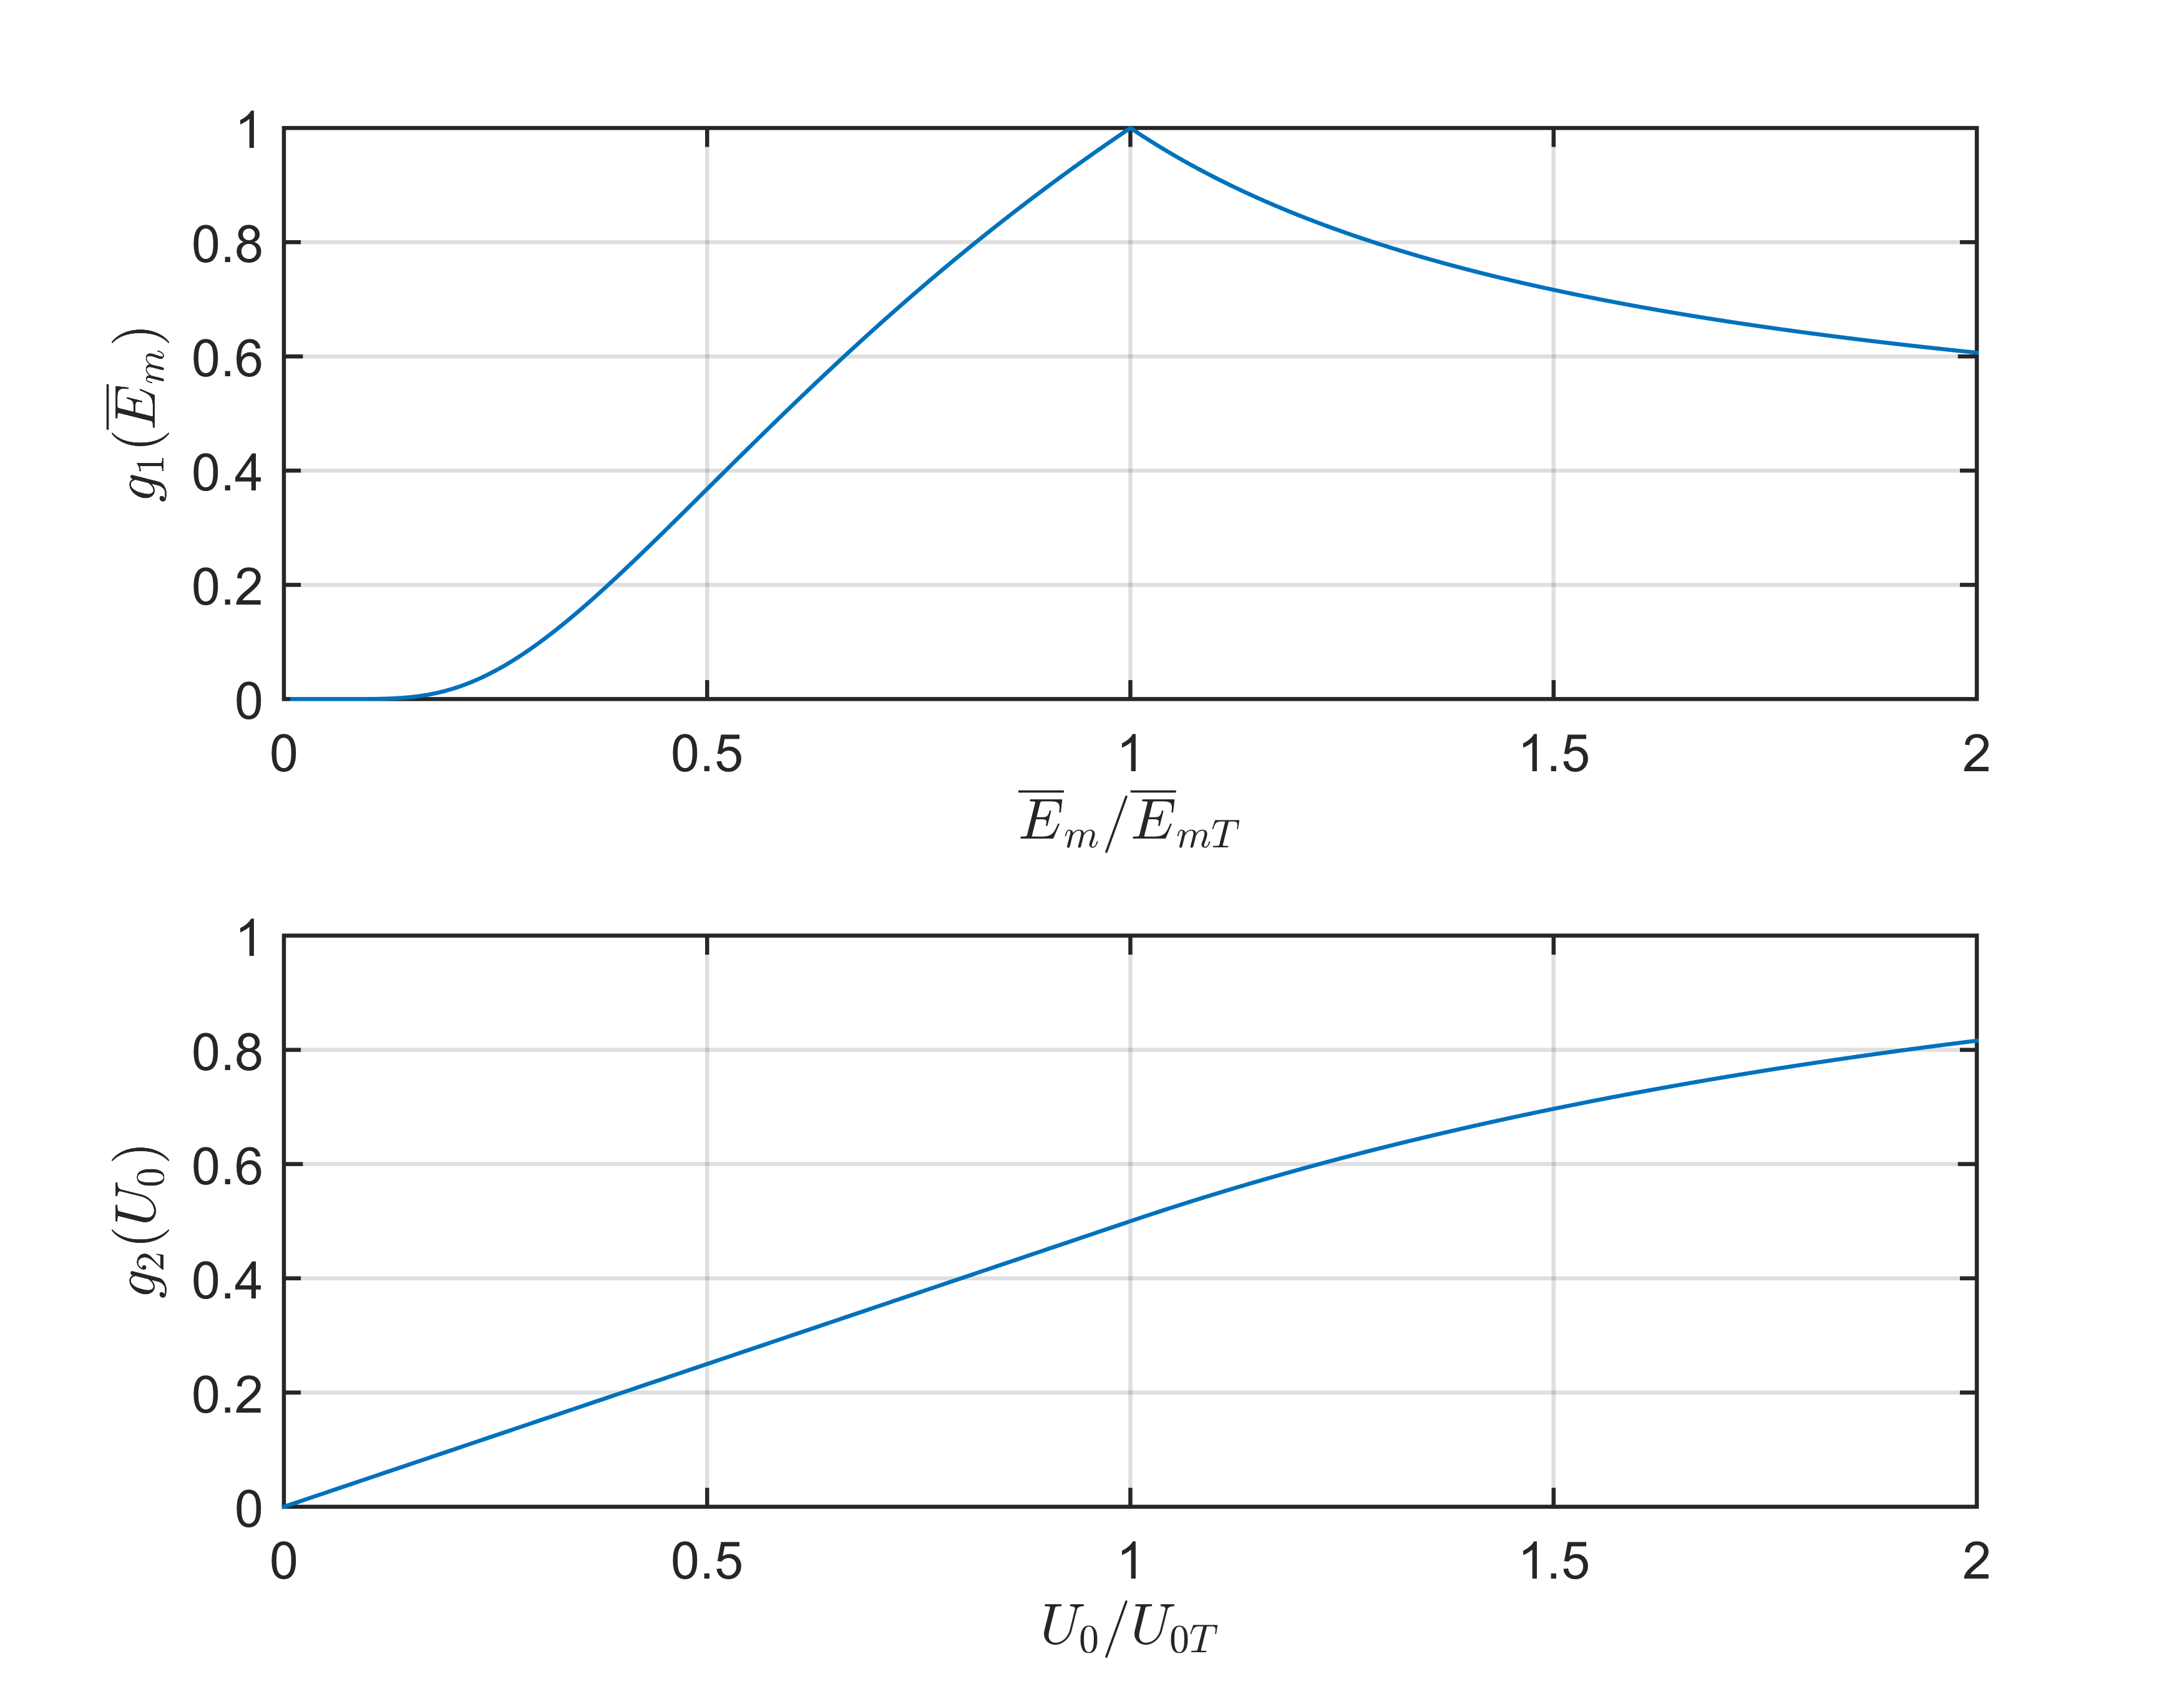
\includegraphics[width=\columnwidth]{obrG1G2}
  \caption{Graphs of parts $g_1\left(\overline{E}_{m}\right)$ and $g_2\left(U_0\right)$ from the fitness function}
  \label{fig:fitV1G1G2}
\end{figure}

The fitness function bellow is currently used in the algorithm. Solutions that does not reach basic requirements of target illuminance or uniformity are valued by length of the chromosome $L$:

\begin{equation}
\label{eq:fitV2EUA}
	f\left(\overline{E}_{m}, U_0\right)= L
\end{equation}

Otherwise the fitness is evaluated by:

\begin{equation}
\label{eq:fitV2EUB}
	f\left(\overline{E}_{m}, U_0\right)= C + \frac{\overline{E}_{mT}}{\overline{E}_{m}} \cdot \frac{U_0T}{U_0}
\end{equation}

\noindent where:
\begin{description}
	\item[$C$] is count of luminaires,
	\item[$\overline{E}_{m}$] is a calculated maintained average value of illuminance,
	\item[$\overline{E}_{mT}$] is a target maintained average value of illuminance,
	\item[$U_0$] is a calculated lighting uniformity,
	\item[$U_{0T}$] is a target lighting uniformity.
\end{description}